\documentclass[11pt,a4paper]{article}

\usepackage[margin=1in, paperwidth=8.3in, paperheight=11.7in]{geometry}
\usepackage{amsfonts}
\usepackage{amsmath}
\usepackage{amssymb} 
\usepackage{enumerate}
\usepackage{enumitem}
\usepackage{fancyhdr}
\usepackage{graphicx}
\usepackage{hyperref}

\begin{document}

\pagestyle{fancy}
\setlength\parindent{0pt}
\allowdisplaybreaks

\renewcommand{\headrulewidth}{0pt}

% Cover page title
\title{Machine Learning - Notes}
\author{Dom Hutchinson}
\date{\today}
\maketitle

% Header
\fancyhead[L]{Dom Hutchinson}
\fancyhead[C]{Machine Learning - Notes}
\fancyhead[R]{\today}

% Enumerate
\setlist[enumerate,1]{label={\roman*)}}

% Counters
\newcounter{definition}[section]
\newcounter{example}[section]
\newcounter{notation}[section]
\newcounter{remark}[section]
\newcounter{theorem}[section]
\newcounter{proof}[section]
\newcounter{proposition}[section]

% commands
\newcommand{\dotprod}[0]{\boldsymbol{\cdot}}
\newcommand{\cosech}[0]{\mathrm{cosech}\ }
\newcommand{\cosec}[0]{\mathrm{cosec}\ }
\newcommand{\sech}[0]{\mathrm{sech}\ }
\newcommand{\blocks}[0]{\mathbb{B}}
\newcommand{\nats}[0]{\mathbb{N}}
\newcommand{\reals}[0]{\mathbb{R}}
\newcommand{\eg}[0]{\textit{e.g.} }
\newcommand{\ie}[0]{\textit{i.e.} }
\newcommand{\integers}[0]{\mathbb{Z}}
\newcommand{\nb}[0]{\textit{N.B.} }
\newcommand{\prob}[0]{\mathbb{P}}
\newcommand{\expect}[0]{\mathbb{E}}
\newcommand{\var}[0]{\mathrm{var}}
\newcommand{\cov}[0]{\mathrm{cov}}
\newcommand{\argmax}[0]{\mathrm{argmax}}
\newcommand{\argmin}[0]{\mathrm{argmin}}
\newcommand{\proved}[0]{$\hfill\square$\\}

\newcommand{\x}[0]{\textbf{x}}
\newcommand{\X}[0]{\textbf{X}}
\newcommand{\mub}[0]{\pmb{\mu}}

\newcommand{\definition}[1]{\stepcounter{definition} \textbf{Definition \arabic{section}.\arabic{definition}\ - }\textit{#1}\\}
\newcommand{\definitionn}[1]{\stepcounter{definition} \textbf{Definition \arabic{section}.\arabic{definition}\ - }\textit{#1}}
\newcommand{\proof}[1]{\stepcounter{proof} \textbf{Proof \arabic{section}.\arabic{proof}\ - }\textit{#1}\\}
\newcommand{\prooff}[1]{\stepcounter{proof} \textbf{Proof \arabic{section}.\arabic{proof}\ - }\textit{#1}}
\newcommand{\example}[1]{\stepcounter{example} \textbf{Example \arabic{section}.\arabic{example}\ - }\textit{#1}\\}
\newcommand{\examplee}[1]{\stepcounter{example} \textbf{Example \arabic{section}.\arabic{example}\ - }\textit{#1}}
\newcommand{\notation}[1]{\stepcounter{notation} \textbf{Notation \arabic{section}.\arabic{notation}\ - }\textit{#1}\\}
\newcommand{\notationn}[1]{\stepcounter{notation} \textbf{Notation \arabic{section}.\arabic{notation}\ - }\textit{#1}}
\newcommand{\proposition}[1]{\stepcounter{proposition} \textbf{Proposition \arabic{section}.\arabic{proposition}\ - }\textit{#1}\\}
\newcommand{\propositionn}[1]{\stepcounter{proposition} \textbf{Proposition \arabic{section}.\arabic{proposition}\ - }\textit{#1}}
\newcommand{\remark}[1]{\stepcounter{remark} \textbf{Remark \arabic{section}.\arabic{remark}\ - }\textit{#1}\\}
\newcommand{\remarkk}[1]{\stepcounter{remark} \textbf{Remark \arabic{section}.\arabic{remark}\ - }\textit{#1}}
\newcommand{\theorem}[1]{\stepcounter{theorem} \textbf{Theorem \arabic{section}.\arabic{theorem}\ - }\textit{#1}\\}
\newcommand{\theoremm}[1]{\stepcounter{theorem} \textbf{Theorem \arabic{section}.\arabic{theorem}\ - }\textit{#1}}

% Table of contents
\tableofcontents
\section*{General}
Lecturer - \href{carlhenrik.ek@bristol.ac.uk}{Carl Henrik Ek}\\
Course Website - \url{http://carlhenrik.com/COMS30007/}\\
Course Repo - \url{https://github.com/carlhenrikek/COMS30007}\\
Course Subreddit - \url{https://www.reddit.com/r/coms30007/}

% Start of content
\newpage

\section{Introduction}

\subsection{Motivation}

\definition{Deductive Reasoning}
A method of reasoning in which the premieses are viewed as supplying \underline{all} the evidence for the truth of the conclusion.\\

\definition{Inductive Reasoning}
A method of reasoning in which the premieses are viewed as supplying \underline{some} evidence for the truth of the conclusion, rather than all the evidence. This allows for the conclusion of the \textit{Inductive Reasoning} to be false.\\

\remark{Free-Lunch Theorem}
There are infinite number of hypotheses that perfectly explain the data. Adding a data point removes an infinite number of possibilities, but still leaves infinite possibilities.\\

\remark{The Task of Machine Learning}
When proposing to use machine learning on a task, one should consider the following questions:
\begin{enumerate}[label=\roman*)]
	\item How can we formulate beliefes ad assumptions mathematically?
	\item How can we connect our assumptions with data?
	\item How can we update our beliefs?
\end{enumerate}

\remark{Useful Models are not always True}
Our goal is to understand realisations of a system. If we can then we can equate our model to the system. It is important to note thtat our model does not need to be perfectly true to be useful.

\subsection{Probability Theory}

\definition{Stochastic/Random Variable}
A variable whose value depends on outcomes of random phenomona.\\
\eg $x\sim\mathcal{N}(0,1)$.\\

\definition{Probability Measure,$\prob$}
A function with signature $\prob:\mathcal{F}\to[0,1]$, where $\mathcal{F}$ is a sample space of rv $X$, and fulfils $\int_{-\infty}^{\infty}\prob(x)dx=1$.\\

\definition{Joint Probability Distribution}
A \textit{Probability Measure} for multiple variables, $\prob:X\times Y\to[0,1]$.\\
Let $n_{ij}$ be the number of outcomes where $X=x_i$ and $Y=y_j$ then
$$\prob(X=x_i,Y=y_j)=\frac{n_{ij}}{\sum_{i,j}n_{ij}}$$

\definition{Marginal Probability Distribution}
A \textit{Probability Measure} for one variable when the sample space is over multiple variables.\\
Let $n_{ij}$ be the number of outcomes where $X=x_i$ and $Y=y_j$ then
$$\prob(X=x_i)=\frac{\sum_jn_{ij}}{\sum_{i,j}n_{ij}}$$

\definition{Conditional Probability Distribution}
A \textit{Probability Measure} for a variable, given another variable has a defined value.
Let $n_{ij}$ be the number of outcomes where $X=x_i$ and $Y=y_j$ then
$$\prob(Y=y_j|X=x_i)=\frac{n_{ij}}{\sum_{j}n_{ij}}$$

\example{Joint, Marginal \& Conditional Probability}
The below image shows two marginals distributions in the bottom-left, $X$, \& top-right, $Y$, their joint distribution in the top-left and a conditional in the bottom right $\prob(Y|X=1)$.\\
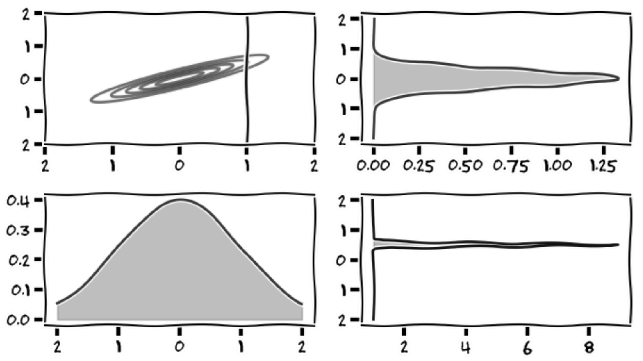
\includegraphics[scale=2]{img/probExamples.png}

\theorem{Product Rule}
For random variables $X$ \& $Y$
$$\prob(X=x,Y=Y)=\prob(Y=y|X=x)\prob(X=x)$$

\theorem{Sum Rule}
For random variables $X$ \& $Y$
$$\prob(X=x)=\sum_j\prob(X=x,Y=y_j)$$

\theorem{Baye's Theorem}
For random variables $X$ \& $Y$
$$\prob(X=x|Y=y)=\frac{\prob(Y=y|X=x)\prob(X=x)}{\prob(Y=y)}$$

\definition{Elements of Bayes' Theorem}
The elements of \textit{Bayes' Theory} can be broken down to explain parts of the model.
$$\underbrace{\prob(\theta|Y)}_{\text{Posterior}}=\frac{\overbrace{\prob(Y|\theta)}^{\text{Likelihood}}\overbrace{\prob(\theta)}^{\text{Prior}}}{\underbrace{\prob(Y)}_{\text{Evidence}}}$$
\begin{tabular}{l|l}
Posterior&Which parameters of the model do I belive produce distributions have generated the data $Y$\\
Likelihood&How likley is the data to come from the model specifely indexed by $\theta$\\
Prior&What distribution do I think parameter $\theta$ has\\
Evidence&How likely do I think data $Y$ is for all models.
\end{tabular}
\nb The \textit{Evidence} normalises this function.\\

\definition{Expectaction Value, $\expect$}
The mean value a random variable will produce from a large number of samples.\\
\begin{tabular}{l|l}
Continuous&Discrete\\\hline
$\expect(X)=\int_{-\infty}^{\infty} x\prob(X)dx$&$\expect(X)=\sum_{-\infty}^{\infty} x\prob(X)dx$\\
$\expect(f(X))=\int_{-\infty}^{\infty} f(x)\prob(X)dx$&$\expect(f(X))=\sum_{-\infty}^{\infty} f(x)\prob(X)dx$
\end{tabular}\\

\definition{Variance}
Describes the amount of spread in the values a single random variable will produce.
$$\var(X)=\expect\left(x-\expect(x))^2\right)=\expect(X^2)-\bigg(\expect(X)\bigg)^2$$

\definition{Covariance}
Describes the joint variability between two random variables.
$$\cov(X,Y)=\expect\bigg(\big(X-\expect(X)\big)\big(Y-\expect(Y)\big)\bigg)$$

\definition{Marginalisation}
The process of summing out the probability of one random variable using its joing probability with another rando variable.
\[\begin{array}{rrcl}
\mathrm{Continuous}&\prob(X=x)&=&\int(X=x,Y=y)dy\\
\mathrm{Discrete}&\prob(X=x)&=&\sum_i\prob(X=x,Y=y_i)
\end{array}\]

\definition{Likelihood Function}
Define $\X\sim f_n(\cdot;\theta^*)$ for some unknown $\theta^*\in\Theta$ and let $\x$ be an observation of $\X$.\\
A \textit{Likelihood Function} is any function, $L(\cdot;\x):\Theta\to[0,\infty)$, which is proportional to the PMF/PDF of the obeserved realisation $\x$.
$$L(\theta;\x):=Cf_b(\x;\theta)\ \forall\ C>0$$
\nb Sometimes this is called the \textit{Observed} Likelihood Function since it is dependent on observed data.\\

\definition{Log-Likelihood Function}
Let $\X\sim f_n(\cdot;\theta^*)$ for some unknown $\theta^*\in\Theta$ and $\x$ be an observation of $\X$.\\
The \textit{Log-Likelihood Function} is the natural log of a \textit{Likelihood Function}
$$\ell(\theta;\x):=\ln f_n(\x;\theta)+C,\ C\in\reals$$

\definition{Maximum Likelihood Estimation}
The \textit{Maximum Likelihood Estimate} is an estimate for a parameter of a probability distribution which is the value which maximises the \textit{Likelihood Function} (or the \textit{Likelihood Function}).
$$\hat{\theta}:=\text{argmax}_\theta L(\theta;\x)$$

\definition{Central Limit Theorem}
The distribution of the sum (or mean) of a large number of independent, identically distributied random variables can be approximated to a normal distribution, regardless of the distributions of the random variables.

\subsection{Conjugate Priors}

\definition{Conjugate Prior}
If we have a \textit{Likelihood Function}, $\prob(X|\theta)$, with a known distribution (\eg Normal) we can choose our \textit{Prior}, $\prob(\theta)$, to be from a distribution which is \textit{Conjugate} to the distribution of the \textit{Likelihood Function}.\\
These are defined in \href{https://en.wikipedia.org/wiki/Conjugate_prior#Table_of_conjugate_distributions}{\textit{tables}}\\

\remark{Why use Conjugate Priors?}
If we have a \textit{Conjugate Prior} then the \textit{Posterior}, $\prob(\theta|X)$, will be in the same distribution family as the \text{Prior} too. We can then work out the distribution of the \textit{Posterior} by passing the parameters of the \textit{Prior} through pre-derived functions
\[\begin{array}{rcl}
\text{Posterior}&\propto&\text{Likelihood}\times\text{Prior}\\
\prob(\theta|X)&\propto&\prob(X|\theta)\times\prob(\theta)
\end{array}\]
\nb - \url{https://en.wikipedia.org/wiki/Conjugate_prior#Table_of_conjugate_distributions}\\

\example{Conjugate Priors}
Consider a scenario where we are flipping a coin. We may have \textit{Likelihood Function} $\theta^x(1-\theta)^{n-x}$. If we choose our \textit{Prior} to be $\theta^{a-1}(1-\theta)^{b-1}$ which is a \textit{Beta Distribution}.\\
Then (after some maths) we find the \textit{Posterior}

\section{Distributions}

\definition{Bernoulli Distribution}
Models an event with a binary outcome (0 or 1) with parameter $p$ st $\prob(X=1)=p$
Let $X\sim\text{Bernoulli}(p)$. Then
\[\begin{array}{rcl}
f_X(x)&=&\begin{cases}
p&, x=1\\
1-p&, x=0\\
0&\text{otherwise}
\end{cases}\\
F_X(x)&=&\begin{cases}
0&,x<0\\
1-p&0\leq x<1\\
1&x\geq1
\end{cases}\\
\expect(X)&=&p\\
\text{Var}(X)&=&p(1-p)
\end{array}\]

\definition{$\beta$-Distribution}
A \textit{$\beta$-Distribution} is a continuous distribution over interval $[0,1]$ which is parameterised by two positive \textit{shape parameters}, $\alpha\ \&\ \beta$. A \textit{$\beta$-Distribution} can be used to encode assumptions as a \textit{Prior}.\\
Let $X\sim\beta(\alpha,\beta)$. Then
\[\begin{array}{rcl}
f_X(x)&=&\dfrac{\Gamma(\alpha+\beta)}{\Gamma(\alpha)+\Gamma(\beta)}x^{\alpha-1}(1-x)^{\beta-1}
\end{array}\]

\example{$\beta$-Distribution}
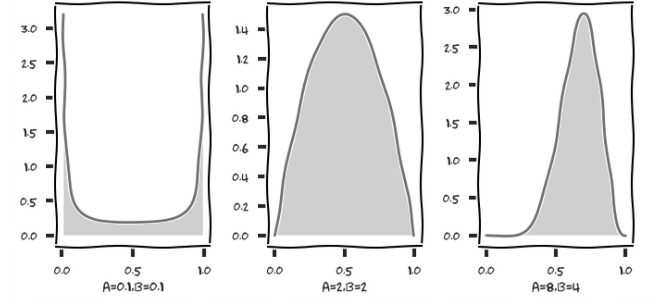
\includegraphics[scale=.6]{img/betaExamples.png}

\definition{Direchlet Distribution}
Let $X\sim\text{Dir}(\pmb{\alpha})$. Then
$$f_X(x):=\dfrac{\Gamma(\alpha_0)}{\Gamma(\alpha_1)\times\dots\times\Gamma(\alpha_N)}\prod_{i=1}^Nx_i^{\alpha_{i-1}}$$

\definition{Exponential Distribution Family}
The \textit{Exponential Distribution Family} is a set of probability distributions which fit the form.
$$\prob(\x|\pmb{\theta})=h(\x)g(\pmb{\theta})e^{\pmb{\theta}^T\textbf{u}(\x)}$$
With conjugate prior
$$\prob(\pmb{\theta}|\pmb{\chi},\nu)=f(\pmb{\chi},\nu)g(\pmb{\chi})^\nu e^{\nu\pmb{\theta}^T\pmb{\chi}}$$

\definition{Multivariate Normal Distribution}
Let $\X\sim\mathcal{N}(\mub,\pmb{\Sigma})$. Then
$$f_\X(\x)=\dfrac{1}{(2\pi)^{N/2}|\pmb{\Sigma}^{1/2}}e^{-\frac{1}{2}(\x-\mub)^T\pmb{\Sigma}^{-1}(\x-\mub)}$$
\nb Also known as \textit{Gaussian Distribution}.

\section{Regression}

\definition{Supervised Learning}
Learning the relationship $f(\cdot)$ between pairs of data $x_i$ and $y_i$ where $y_i=f(x_i)$.\\

\remarkk{Summary of Regression}
\begin{itemize}
	\item[Linear Regression] We are limited to lines
	\item[Basis Functions Regression] We can use non-linear functions, but it is hard to determine how many \& what basis functions should be used. The prior is hard to interpret.
	\item[Kernel Regression] The complexity is defined by the data (Good) but there is no uncertainty in our estimate.
\end{itemize}

\subsection{Linear Regression}

\definition{Linear Regression}
\textit{Linear Regression} is the process of taking a set of data points \& producing a linear relationship between a dependent varaible \& one of more explanatory variables.\\
Let $\x\in\reals^n$ be a set of observed values from $n$ explanatory variables \& $\textbf{a}\in\reals^n+1$ be a set of parameters. Then we predict the value of the dependent variable to be
$$y(\x,\textbf{a})=a_0+\sum\limits_{i=0}^na_{i+1}x_i$$

\remark{Limitation of Linear Regression}
The formula defined in \textbf{Definition 3.1} is a linear function of the coefficients defined by $\textbf{a}$ \textbf{and} the observed values of $\x$ this limits the relationships we can model between elements of $\x$. The model can be extended to avoid this using \textit{Basis Functions}.\\

\definition{Linear Regression - Basis Functions}
We can extend \textit{Linear Regression} to include \textit{Basis Functions} so that relationships between explanatory variables can be modelled.\\
Let $\x\in\reals^n$ be a set of observed values from explanatory variables, $\textbf{a}\in\reals^{m}$ be a set of coefficients (weightings), and $\pmb{\phi}:\reals^n\to\reals^{m-1}$ be a set of basis functions. Then we can predict the dependent variable to be
$$y(\x,\textbf{a})=a_0+\sum_{i=1}^ma_i\phi_{i-1}(\x)$$

\remark{Linear Regression - Basis Function}
To simplfy the equation used in \textbf{Definition 3.2} we can define $\pmb{\phi}:\reals^n\to\reals^m$ with $\phi_0(\x)$. Then
$$y(\x,\textbf{a})=\sum_{i=0}^ma_i\phi_i(\x)=\textbf{a}^T\pmb{\phi}(\x)$$

\proposition{Noise}
We will often introduce the concept of \textit{Noise} into a \textit{Linear Regression} model. Typically we assume noise to be modelled by a zero-mean Normal distribution with precision $\beta$, $\varepsilon\sim\text{Normal}(0,\beta^{-1})$, so
$$t:=y(\x,\textbf{a})=\textbf{a}^T\pmb{\phi}(\x)+\varepsilon$$
From this we can derive a likelihood
$$\prob(t|\x,\textbf{a},\beta)\sim\text{Normal}(t|\mu=y(\x,\textbf{a}),\sigma^2=\beta^{-1})=\text{Normal}(t|\mu=\textbf{a}^T\pmb{\phi}(\x),\sigma^2=\beta^{-1})$$
If we have a series of sets of observations, $\X\in\reals^{m\times n}$, then
$$\prob(\textbf{t}|\X,\textbf{a},\beta)\sim\prod\limits_{i=1}^m\text{Normal}(t_i|\mu=\textbf{a}^T\pmb{\phi}(\x_i),\sigma^2=\beta^{-1})$$
%TODO what is precision v variance in normal distribution

\definition{Maximum Likelihood Estimate}
A \textit{Maximum Likelihood Estimate} is estimating the value of a parameter to be the most likely, according to our \textit{Likelihood Function}.\\

\remark{Finding Maximum Likelihood Estimate}
Suppose we have a defined \textit{Likelihood Function} $\prob(\textbf{t}|\X,\textbf{a},\beta)$ and we want to find \textit{Maximum Likelihood Estimates} for parameters $\textbf{a}$. Then
\begin{enumerate}[label=\roman*)]
	\item Define the \textit{Likelihood Function}, $\prob(\textbf{t}|\X,\textbf{a},\beta)$.
	\item Take the natural log, $\ln\prob(\textbf{t}|\X,\textbf{a},\beta)$.
	\item Take the derivative wrt $\textbf{a}$, $\frac{\partial}{\partial\textbf{a}}\ln\prob(\textbf{t}|\X,\textbf{a},\beta)$.
	\item Set the derivatite to $0$, $\frac{\partial}{\partial\textbf{a}}\ln\prob(\textbf{t}|\X,\textbf{a},\beta)=0$.
	\item Solve to find the stationary point of $\textbf{a}$.
	\item Check this stationary point is a maximum, if it is then it is a \textit{Maximum Likelihood Estimate}
\end{enumerate}

\example{Maximum Likelihood Estimate}
Here I shall find the \textit{Maximum Likelihood Estimate} for $\textbf{a}$
\[\begin{array}{rrcl}
&\prob(\textbf{t}|\X,\textbf{a},\beta)&\sim&\prod\limits_{i=1}^m\text{Normal}(t_i|\textbf{a}^T\pmb{\phi}(\x_i),\beta^{-1})\\
&&=&\prod\limits_{i=1}^m\dfrac{1}{\sqrt{2\pi\beta^{-1}}}e^{-\frac{1}{2}\beta(t_i-\textbf{a}^T\pmb{\phi}(x_i))^2}\\
&&=&\left(\frac{\beta}{2\pi}\right)^{\frac{m}{2}}e^{-\frac{\beta}{2}\sum\limits_{i=1}^m(t_i-\textbf{a}^T\pmb{\phi}(x_i))^2}\\
\implies&\ln\prob(\textbf{t}|\X,\textbf{a},\beta)&=&\frac{m}{2}(\underbrace{\ln(\beta)}_{\text{Noise Precision}}-\underbrace{\ln(2\pi)}_{\text{Constant}})-\underbrace{\frac{\beta}{2}\sum\limits_{i=1}^m(t_i-\textbf{a}^T\pmb{\phi}(x_i))}_{\text{Error}}\\
\implies&\frac{\partial}{\partial\textbf{a}}\ln\prob(\textbf{t}|\X,\textbf{a},\beta)&=&\beta\sum\limits_{i=1}^2(\textbf{t}_i-\textbf{a}^T\pmb{\phi}(\x_i))\pmb{\phi}(x_i)^T\\
\text{Setting}&0&=&\frac{\partial}{\partial\textbf{a}}\ln\prob(\textbf{t}|\X,\textbf{a},\beta)\\
\implies&0&=&\beta\sum\limits_{i=1}^2(\textbf{t}_i-\textbf{a}^T\pmb{\phi}(\x_i))\pmb{\phi}(x_i)^T\\
&&=&\left(\sum\limits_{i=1}^m\textbf{t}_i\pmb{\phi}(\x_i)^T\right)-\textbf{a}^T\left(\sum\limits_{i=1}^m\pmb{\phi}(\x_i)\pmb{\phi}(\x_i)^T\right)\\
\implies&\textbf{a}_{MLE}&=&\left(\pmb{\phi}(\X)^T\pmb{\phi}(\X)\right)^{-1}\pmb{\phi}(\X)^T\textbf{t}
\end{array}\]

\theorem{Variance of Posterior}
Let $\alpha$ be the parameter of the prior, $\beta$ be the parameter for the likelihood and $\X$ be the observed values from the predictor variables.
%TODO not sure of these definitions
\[\begin{array}{rcl}
s_n&=&(I\alpha+\beta \X^T\X)^{-1}\\
&=&\left(I\alpha+\beta\begin{pmatrix}
\sum\limits_{i=1}^n1&\sum\limits_{i=1}^nx_i\\
\sum\limits_{i=1}^nx_i&\sum\limits_{i=1}^nx_i^2
\end{pmatrix}\right)^{-1}\\
&=&\begin{pmatrix}
\beta n+\alpha&\beta\sum\limits_{i=1}^nx_i\\
\beta\sum\limits_{i=1}^nx_i&\alpha+\beta\sum\limits_{i=1}^nx_i^2
\end{pmatrix}^{-1}\\
&=&\dfrac{1}{(\beta n+\alpha)\left(\alpha+\beta\sum\limits_{i=1}^nx_i^2\right)-\left(\beta\sum\limits_{i=1}^nx_i\right)^2}\begin{pmatrix}
\alpha+\beta\sum\limits_{i=1}^nx_i^2&-\beta\sum\limits_{i=1}^nx_i\\
-\beta\sum\limits_{i=1}^nx_i&\beta n+\alpha
\end{pmatrix}\\
&&\text{Assume data is centred so }\sum\limits_{i=1}^nx_i=0\\
&=&\dfrac{1}{(\beta n+\alpha)\left(\alpha+\beta\sum\limits_{i=1}^nx_i^2\right)}\begin{pmatrix}
\alpha+\beta\sum\limits_{i=1}^nx_i^2&0\\
0&\beta n+\alpha
\end{pmatrix}\\
&=&\begin{pmatrix}
\dfrac{1}{\beta n+\alpha}&0\\
0&\dfrac{1}{\alpha+\beta\sum\limits_{i=1}^nx_i^2}
\end{pmatrix}
\end{array}\]

\theoremm{Mean of Posterior}
Let $\alpha$ be the parameter of the prior, $\beta$ be the parameter for the likelihood, $\X$ be the observed values from the predictor variables and $\textbf{t}$ be the observed values for the dependent variable.
\[\begin{array}{rcl}
m_n&=&(\alpha I+\beta \X^T\X)^{-1}\beta \X^T\textbf{t}\\
&=&s_n\beta\X^T\textbf{t}\\
&=&\beta s_n\begin{pmatrix}
1&\dots&1\\
x_1&\dots&x_n
\end{pmatrix}
\begin{pmatrix}
t_1\\
\vdots\\
t_n
\end{pmatrix}\\
&=&\beta s_n\begin{pmatrix}
\sum\limits_{i=1}^nt_i\\
\sum\limits_{i=1}^nt_ix_i
\end{pmatrix}\\
&&\text{Assume data is centred so }\sum\limits_{i=1}^nx_i=0\\
&=&\beta\begin{pmatrix}
\dfrac{1}{\beta n+\alpha}&0\\
0&\dfrac{1}{\alpha+\beta\sum\limits_{i=1}^nx_i^2}
\end{pmatrix}\begin{pmatrix}
\sum\limits_{i=1}^nt_i\\
\sum\limits_{i=1}^nt_ix_i
\end{pmatrix}\\
&=&\begin{pmatrix}
\dfrac{\beta\sum_{i=1}^nt_i}{\beta n+\alpha}\\
\dfrac{\beta\sum_{i=1}^nt_ix_i}{\alpha+\beta\sum_{i=1}^nx_i^2}
\end{pmatrix}
\end{array}\]

\proposition{Prediction}
Suppose we are given as inputs to the model: $\X$ observations from the predictor variables, $\textbf{t}$ observations from the dependent variable; $\alpha$, parameter for the prior; and $\beta$, parameter for the likelihood.\\
If we now want to predict the value $\hat{t}$ at position $\hat{\x}$ we want to solve
$$\prob(\hat{t}|\hat{\x},\textbf{t},\X,\alpha,\beta)=\int\prob(\hat{t}|\hat{\x},\textbf{a},\beta)\prob(\textbf{a}|\textbf{t}|\X,\alpha,\beta)d\textbf{a}$$
where $\textbf{a}$ is the coefficient for weighting each parameter.

\subsection{Dual Linear Regression}

\definition{Kernel}
A \textit{Kernel} is a function that defines an inner-produce in some space.\\
Let $\x$ be a vector in the orignal space \& $\phi(\cdot)$ map from the original space to the kernel space. Then the \textit{Kernel Function} is defined as
$$k(\x_i,\x_j):=\phi(\x_i)^T\phi(\x_j)$$

\remark{Usefulness of Kernels}
It is generally easier to define the inner-product of a space than to define a space \& kernels allow us to never have to realise a space. This allows us to work with infinite dimensional spaces.\\
\nb The space defined by the \textit{Kernel} is called the \textit{Induced Space}.\\

\definition{Kernel Regression}
\textit{Kernel Regression} is the act of performing a linear regression in an \textit{Induced Space}.\\
Let $\X$ \& $\textbf{t}$ be  training data, $\lambda$ be a parameter for noise, $\hat{\x}$ be an unseen data point which we wish to predicit a value $\hat{y}$ for. Then
$$\hat{y}(\hat{\x})=k(\hat{\x},\x)(k(\X,\X)+\lambda I)^{-1}\textbf{t}$$

\remark{Usefulness of Kernel Regression}
Note that the problem is linear in the \textit{Induced Space} but not in the original space, thus allowing us to learn non-linear functions using lines.\\


\remark{Changing Basis}
Some data is clearly non-linear \& it may be helpful to transform it into another basis where linear regression is possible.\\
\eg If the data appearas to fit a circle in a cartesian basis, it can be translated into polar co-ordinates which should be linear.\\
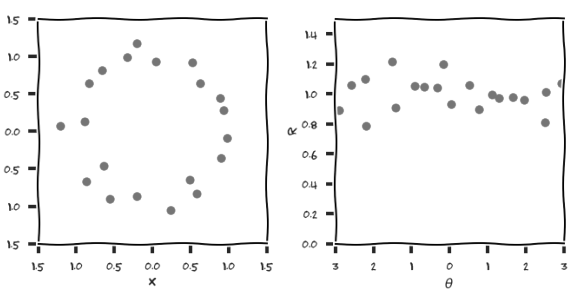
\includegraphics[scale=.4]{img/changeBasis.png}

\proposition{Changing Basis}
Let $\textbf{a}$ be weightings for observed parameters and $\x$ be a set of observed parameters.\\
Suppose we want to change the basis of $\x$, if we have a function $\phi:\mathcal{X}\to\mathcal{Z}$ which can do this then we predict $y$ as
$$t=\textbf{a}^T\phi(\x)=\textbf{a}^T\textbf{z}$$

\definition{Dual Linear Regression}
Standard \textit{Linear Regression} is defined as a linear combination of columns. \textit{Dual Linear Regression} is a linear combination of the inner product of a new data point with each of the training data, this allows it to consider combinations of data points.\\

\remark{Intution of Dual Regression}
\textit{Dual Regression} can be considered as describing an unseen data points as a combination of seen ones. \ie Has the shape of a rhino, fur of a tiger, ...\\

\proposition{Dual Linear Regression Steps}
To perform a \textit{Dual Linear Regression} perform the following
\begin{enumerate}[label=\roman*)]
	\item Formulate Posterior, $\prob(\theta|\X)$;
	\item Find stationary point of posterior;
	\item Re-write the coefficients $\textbf{a}$ in terms of the data;
	\item Perform Kernel regression.
\end{enumerate}
%TODO formulae & better explanation of process

\remark{Useful Kernels}
Not all functions can be used as \textit{Kernels}. Some that can, and can be useful,
\begin{enumerate}[label=\roman*)]
	\item Kernelised Euclidean Distance $\|\phi(\x_i)-\phi(\x_j)\|^2=k(\x_i,\x_i)-2k(\x_i,\x_j)+k(\x_j,\x_j)$
	\item Exponented Quadratic $k(\x_i,\x_j)=\sigma^2 e^{-\frac{1}{2\ell^2}(\x_i-\x_j)^T(\x_i-\x_j)}$.
\end{enumerate}

\remarkk{Limitations of Linear/Dual Regression}
\begin{enumerate}[label=\roman*)]
	\item No uncertainty in our observed outputs;
	\item No uncertainity in our mapping;
	\item We have to make assumptions over the space of functions
\end{enumerate}

\subsection{Gaussian Processes}

\remark{Motivation}
Here we want to introduce uncertainty into our observed outputs \& mappings. This means that instead of outputting a discrete value we return a probability distribution. Now we can consider a few more features for our observations, such as how much does observing a value at $\x_0$ tell us about an observation at $\x_1$.\\
\nb In the image before we have an observation for $x=-2$ and three marginals for $x=-2,3,6$ which our observation has a decreasing affec on, as distance increases.\\
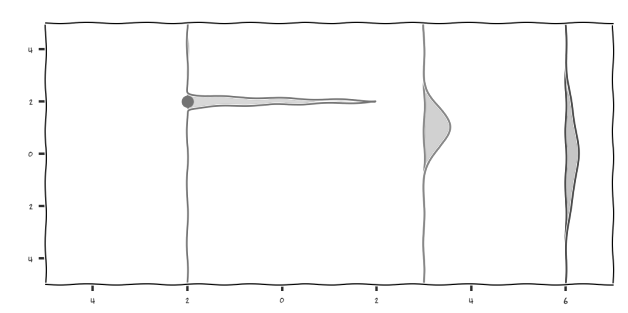
\includegraphics[scale=1]{img/decay.png}

\definition{Gaussian Process}
A \textit{Gaussina Process} is a generalisation of random variables into an infinite number of \textit{Gaussian Distributions}. The specific process is defined by a mean function $\mu(\cdot)$ and a co-variance function function $k(\cdot)$.
$$\prob(f_1,f_2,\dots|\x,\pmb{\theta})\sim\mathcal{GP}\left(\mu(\x),k(\x,\x)\right)=\text{Normal}\left(\begin{pmatrix}
\mu(x_1)\\\mu(x_2)\\\vdots
\end{pmatrix},\begin{pmatrix}
k(x_1,x_1)&k(x_1,x_2)&\dots\\
k(x_2,x_1)&k(x_2,x_2)&\dots\\
\vdots&\vdots&\ddots
\end{pmatrix}\right)$$
\nb \textit{Gaussian Processes} is non-parameteric.\\

\remark{Covariance Function}
The \textit{Covaraince Function} of a \textit{Gaussian Process} defines how much an observation at $\x_0$ affects our prediction for $\x_1$. The greater the covariance values (Not on the main diagonal) the more an observation tells us. We can define the \textit{Covariance Functions} to vary with distance \& other factors.
$$\text{Very little effect}=\begin{pmatrix}
1&.1\\
.1&1
\end{pmatrix}.\quad\text{A lot of effect}=\begin{pmatrix}
1&.9\\
.9&1
\end{pmatrix}$$

\remark{Sampling from a Gaussian Process}
When we take a sample from a \textit{Gaussian Process} we are given a function which fits the distributions defined the \textit{Gaussian Process}.\\

\example{Sampling from a Gaussian Process}
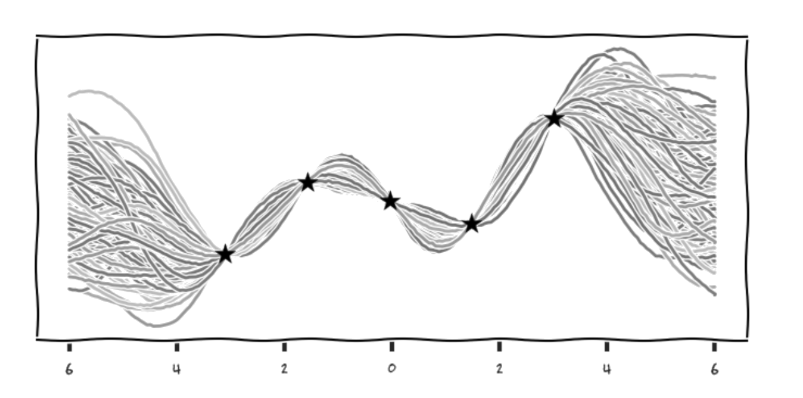
\includegraphics[scale=.7]{img/samplingGaussianProccess.png}

\proposition{Gaussian Process - Posterior, No Noise}
Let $\textbf{f},\X$ be training data, $f^*,\x^*$ be training data and $k$ be the co-variance function. We have %TODO
\[\begin{array}{rcl}\begin{pmatrix}
\textbf{f}\\
f^*
\end{pmatrix}&\sim&\text{Normal}\left(\begin{pmatrix}
\textbf{0}\\
0
\end{pmatrix},\begin{pmatrix}
k(\X,\X)&k(\X,\x^*)\\
k(\x^*,\X)&k(\x^*,\x^*)
\end{pmatrix}\right)\\
\prob(f^*|\x^*,\X,\textbf{f})&\sim&\text{Normal}\bigg(k(\x^*,\X)^Tk(\x^*,\X)^{-1}\textbf{f},\ k(\x^*,\x^*)-k(\x^*,\X)^Tk(\X,\X)^{-1}k(\X,\x^*)\bigg)
\end{array}\]

\proposition{Gaussian Process - Posterior, Noise}
Let $\textbf{f},\X$ be training data, $f^*,\x^*$ be training data and $k$ be the co-variance function.\\ Define $\textbf{y}_i=f_i+\varepsilon$ where $\varepsilon\sim\text{Normal}(0,\sigma^2I)$ We have %TODO
\[\begin{array}{rcl}\begin{pmatrix}
\textbf{y}\\
f^*
\end{pmatrix}&\sim&\text{Normal}\left(\begin{pmatrix}
\textbf{0}\\
0
\end{pmatrix},\begin{pmatrix}
k(\X,\X)+\sigma^2I&k(\X,\x^*)\\
k(\x^*,\X)&k(\x^*,\x^*)
\end{pmatrix}\right)\\
\prob(f^*|\x^*,\x,\textbf{y},\sigma^2)&\sim&\text{Normal}\bigg(k(\x^*,\x)^T(k(\x,\x)+\sigma^2I)^{-1}\textbf{y},\ k(\x^*,\x^*)-k(\x^*,\x)^T(k(\x,\x)+\sigma^2I)^{-1}k(\x,\x^*)\bigg)
\end{array}\]

\example{Noisy Gaussian Process}
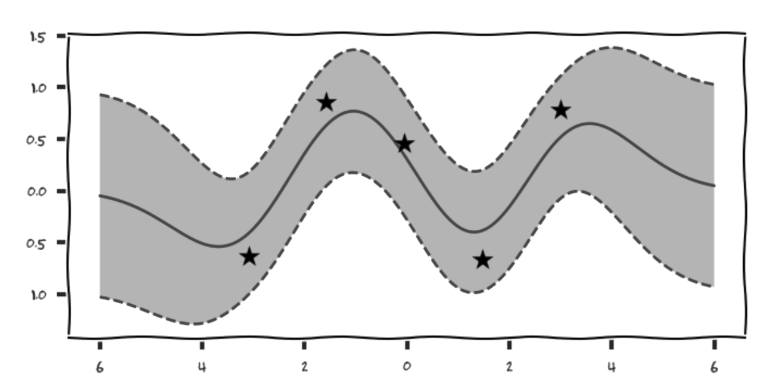
\includegraphics[scale=.7]{img/noisyGaussianProcess.png}

\section{Unsupervised Learning}
%TODO go through NotesLecturer & slides

\definition{Unsupervised Learning}
In \textit{Unsupervised Learning} we are given only the ouput data \& are tasked with deriving the underlying properties of each event.\\
\ie Given $y=f(x)$ recover both $f(\cdot)$ \& $x$.

\section{Bayesian Optimisation}

\remark{Importance of Uncertainty}
Note that we can have $\hat{x}=argmax_xp(x)=\text{argmax}_xq(x)$ but $p(\hat{x})\neq q(\hat{x})$. Due to this we need to introduce uncertainty about the value of $x$ so that we can weight out outcomes accordingly.\\
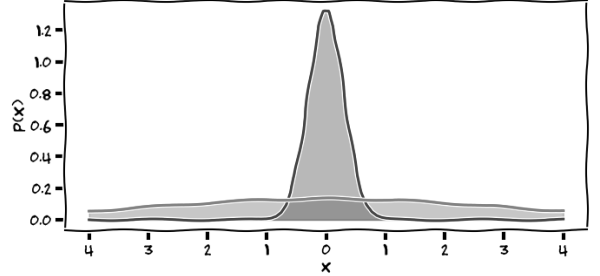
\includegraphics[scale=.4]{img/uncertainty.png}

\definition{Optimisation}
\textit{Optimisation} is the process of finding the best outcome for a problem.\\

\remark{Optimisation}
Classically \textit{Optimisation} is seen as $\hat{x}=\argmin_xf(x)$ however we typically have an objective function that we do not know explicitly, but are able to test. Since testing in real life situations (\eg Medical Trials) are expensive we want to minimise the number required to achieve a good level of certainty.\\

\definition{Global Optimisation}
\textit{Global Optimisation} is the set of techniques for finding $x_M=\argmin_{x\in\mathcal{X}}f(x)$ where $\mathcal{X}$ is a bounded domain (reducing the amount of testing required) and $f$ is not known explicitly. It is possible that evaluations of $f$ are noisy.\\

\propositionn{Bayesian Optimisation}
\begin{enumerate}[label=\roman*)]
	\item Choose a prior over the space of possible objective functions, $f$.
	\item Combine the prior \& likelihood to get a posterior over the space.
	\item Use the posterior to choose a set of evaluations according to a \textit{strategy}.
	\item Add new data, update posterior \& re-evaluate.
	\item Repeat until budget is gone
\end{enumerate}

\proposition{Na\"ive Strategies for Global Optimisation}
Below are some na\"ive \textit{Global Optimisation} stategies
\begin{enumerate}[label=\roman*)]
	\item Implicity knowledge, ask a SME;
	\item Grid Search, test the domain at regular intervals; and,
	\item Random Sampling.
\end{enumerate}

\remark{Interpretting Bayesian Optimisation}
We cannot solve the direct problem $x_M=\argmin_{x\in\mathcal{X}}f(x)$ but can solve $x_{n+1}=\argmin_{x\in\mathcal{X}}\alpha(x;D_n,M_n)$ where $\alpha$ is an \textit{acquisition function}, $D_n$ is the samples taken in the first $n$ steps \& $M_n$ is %TODO

\remark{Exploration v Exploitation}
When considering strategies for \textit{Bayesian Optimisation} we need to consider how we approach \textit{Exploration} (Testing new areas) \& \textit{Explotation} (Investigating areas which seem good). A \textit{Acquisition Function} can be defined which returns the expected gain in information if a sample was to be taken at $x$.\\

\definition{Expected Improvement}
\textit{Expected Improvement} is an \textit{Acquistion Function}.\\
Let $\x$ be a point in the domain, $\theta$ be parameters of the distribution and $X$ be data we already know. Then
$$EI(\x;\theta,X):=\int\max(0,y_{best}-y)\prob(y|\x,\theta,X)dy$$
We should then sample at $\x$ where $EI(\x)\geq EI(\x')\ \forall\ x'\in\mathcal{X}$ since this point offers the greatest information gain.\\
\nb $y_{best}$ is the best value for $y$ we have found so far. \ie The value we are trying to improve.\\
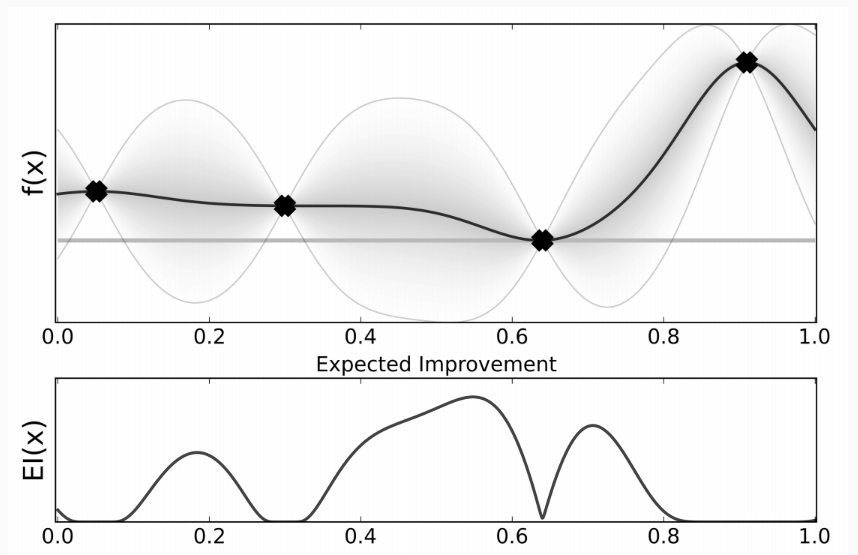
\includegraphics[scale=.4]{img/expectedImprovement.png}

\definition{Thomson Sampling}
\textit{Thomson Sampling} is an \textit{Acquistion Function}.\\
Let $\x$ be a point in the domain, $\theta$ be parameters of the distribution and $X$ be data we already know. Then
$$T(\x;\theta,X):=\prob(y|\x,\x,\theta,X)$$
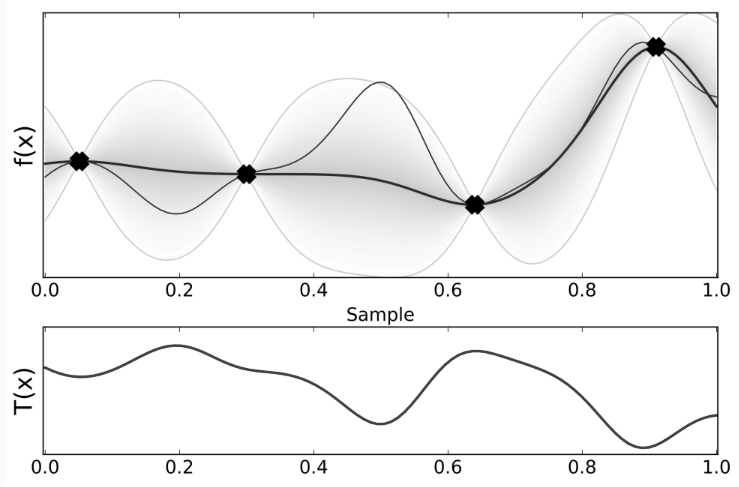
\includegraphics[scale=.4]{img/thomsonSampling.png}

\section{Evidence}

\definition{Evidence}
\textit{Evidence} is part of \textit{Bayes' Theorem}, if models the likelihood of seeing the data we have been given, regardless of parameters.
$$\prob(X)=\int\prob(Y|\theta)\prob(\theta)d\theta$$

\proposition{Using the Evidence}
If we have multiple models we can test them against out \textit{Evidence} \& then choose the model with the greatest accuracy.\\

\remark{Evidence \& Regression Models}
The way we model the \textit{Evidence} depends upon what sort of regression we are doing. Evidence is strongest at points where the lines intersect.\\

\remark{Model Selection - Rule of Thumb}
When choosing a model you should the simplest model which can explain the data.\\
\nb Essentially Occam's Razor.\\
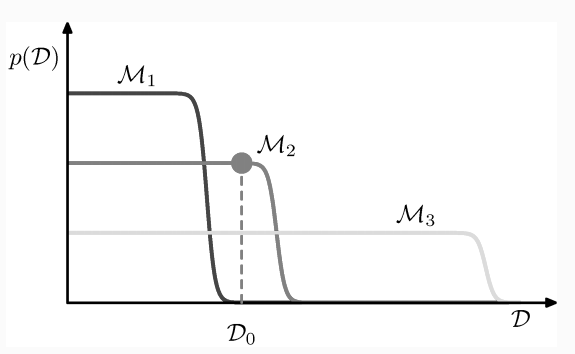
\includegraphics[scale=.5]{img/mackay.png}

\section{Graphical Models}

\definition{Graphical Models}
\textit{Graphical Models} are graphics which show dependency between elements of a model. This dependecy is the minimal factorisation of the joint distribution. \textit{Graphical Models} have several elements
\begin{itemize}
	\item[-] Node - Random  Variable or realisation;
	\item[-] Edge - A stochastic relationship
	\item[-] Plate - A product
\end{itemize}
\textit{Graphical Models} can be directed graphs, often known as \textit{Bayesian Networks}, or undirected, known as \textit{Markov Random Field}.\\

\example{Graphical Model}
The below graphic model shows that $\x \& \textbf{y}$ form a product (ie $x_i$ relates to $y_i$ but not $y_j$ for $i\neq j$) and that $\x$ depends on $c$ \& $\textbf{y}$ depends on $\x$.\\
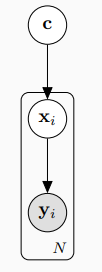
\includegraphics[scale=.5]{img/graphicalModel1.png}

\example{Factorisation of a Directed Graph}
The below \textit{Graphical Model} encodes the factorisation
$$\prob(x_1,\dots,x_7)=\prob(x_1)\prob(x_2)\prob(x_3)\prob(x_4|x_1,x_2,x_3)\prob(x_5|x_1,x_3)\prob(x_6|x_4)\prob(x_7|x_5,x_4)$$
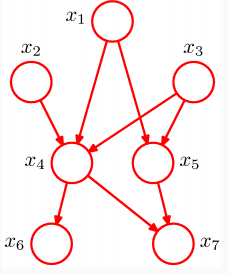
\includegraphics[scale=.5]{img/graphicalModel2.png}\\
\nb We pair each node with its direct parents.\\

\example{Directed Graph with Constants}
We can include \textit{Constants} in a \textit{Graphical Model} as nodes without a circle.\\
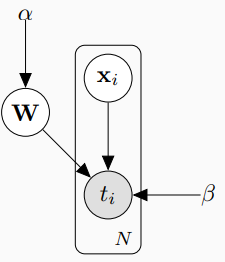
\includegraphics[scale=.5]{img/graphicalModel3.png}

\proposition{Explaining Away}
\textit{Explaining Away} is the process of breaking down a feature into multiple features in such a way that you isolate a particular variance of that feature. This is useful as we may not know much about the original feature but a lot about the sub-features.\\

\example{Explaining Away}
Say you have an image you may wish to break it down into objects, positions \& orientations so that the object variable \textit{explains aways} variance associated with objects from the image. Positions \& orientations will contain no information about the objects. This can be considered as an integral
$$\prob(\text{Image})=\int\prob(\text{Image}|\text{Object,Position,Orientation})\prob(\text{Object})\prob(\text{Position})\prob(\text{Orientation})$$

\proposition{Hierarchical Knowledge}
We can extent the idea of \textit{Explaining Away} by applying it to the sub-features we have produced. If we keep applying this (in a linear fashion) until we find a sub-$\dots$-sub-feature that we have knowledge about then we have utilised a \textit{Hierarchical Knowledge}.\\
This is analogous to defining lots of relationships between features st many features can be explained by a few (in a linear fashion).\\

\section{Non-Parametric Models}

\definition{Non-Parameteric Models}
\textit{Non-Parameteric Models} do not have a specified \textit{a Priori} but are instead determined by the data. This does not mean \textit{Non-Parameteric Models} have no parameters but rather the number they have is not fixed \& their values are not pre-defined. \textit{Non-Parameteric Models} cope in an infinite dimenional parameter space.\\

\definition{Nearest-Neighbour Classifier}
A \textit{Nearest-Neighbour Classifier} takes in a series of training observations \& then when given a test observation simply assigns it to the class of its nearest-neighbour from the training observations.\\
\nb \textit{Nearest-Neighbour Classifier}s consider all features equally, at high dimension irrelevant features may be given too much weight.\\

\definition{$k$-Nearest-Neighbour Classifier}
A \textit{$k$-Nearest Neighbour Classifier} is an extension of the \textit{Nearest Neighbour Classifier}. Instead of just considering the nearest neighbour, it considers the $k$ nearest neighbours to the test observation \& assigns the test observation to the majority class of these $k$ training observations.\\

\definition{Gaussian Mixtures Method}
\textit{Gaussian Mixtures Method} is a \textit{Non-Parameteric Model} which implements \textit{Soft Clustering}. By specifing the number of clusters we want to produce, $k$, we can apply the \textit{Expectation-Maximisation} algorithm to produce $k$ gaussian distributions which represent $k$ different clusters within the data.
\begin{enumerate}[label=\arabic*)]
	\item Initialise random means for each cluster $\mu_1(1),\dots,\mu_k(1)$.
	\item\textit{Estimation Step}\\
	$\forall\ x_i\ \forall\ j\in[1,k]$ set $z_{ij}(t):=\expect\big(z_{ij}|x_j,\mu_j(t)\big)$.\\
	Normalise $z_{i1},\dots,z_{ik}$ st $\sum_{i=1}^kz_{ij}=1$
	\item \textit{Maximisation Step}\\
	$\forall\ j\in[1,k]$ set $\mu_j(t+1):=\dfrac{\sum_{i=1}^nz_{ij}(t)x_i}{\sum_{i=1}^nz_{ij}(t)}$
\end{enumerate}

\remark{Gaussian Processes}
\textit{Gaussian Processes} are \textit{Non-Parameteric}.\\

\definition{Generative Model}
A \textit{Generative Model} is a model which given a set of outcomes $y$ it wishes to derive the data which formed it, $X$.
$$\prob(X|Y=y)$$

\example{Constructing a Generative Model}
Consider a scenario where we want to model the topics which occur in a text.\\
We will define a "topic distribution" which gives the likelihood of each topic, independent of the data.\\
To consider words we define a "word-topic distribution" which gives the likelihood of a given topic being discussed given a certain word has occurred.\\
We can specify a generative model for text data by
\begin{enumerate}[label=\roman*)]
	\item Choose a random distribution over topics
	\item Randomly choose a topic from the topic distribution
	\item Randomly choose a word from word distribution of that topic
\end{enumerate}
Let $w_{d,n}$ be the $n^\text{th}$ word in the $d^\text{th}$ document, $\beta_k$ be the topic-word distribution of the $k^\text{th}$ topic, $\theta_d$ be the topic distribution for the $d^\text{th}$ document and $z_{d,b}$ be the true topic for $n^\text{th}$ word in the $d^\text{th}$ document.\\
Then we have joint distribution
$$\prob(w,z,\theta,\beta)=\underbrace{\prod_{k=1}^K\prob(\beta_k)\underbrace{\prod_{d=1}^D\prob(\theta_k)\underbrace{\prod_{n=1}^N\prob(w_{d,n}|\beta,z_{d,n})\prob(z_{d,n}|\theta_d)}_{\text{word}}}_{\text{document}}}_{\text{corpus}}$$

\subsection{Dirichlet Process}

\definition{Dirichlet Distribution}
The \textit{Dirichlet Distribution} is a generalisation of the $\beta$ distibution \& is the conjugate prior of the \textit{Multinominal Distribution}.
$$\text{Dir}(\pmb{\mu}|\alpha)=\frac{\Gamma(\alpha_0)}{\Gamma(\alpha_1)\cdot\dots\cdot\Gamma(\alpha_K)}\prod_{k=1}^K\mu_k^{\alpha_{k}-1}$$

\definition{Dirichlet Process}
A \textit{Dirichlet Process} is an infinite dimensional generalisation of a \textit{Dirichlet Distribution}. It generates a partioning of (possibly) infinite number of elements. It is unintuitive to define a \textit{Dirichlet Process} mathematically \& thus we write it constructively.\\

\definition{Chinese Restaurant Process}
Consider having an infinite number of tables (clusters) \& dishes (labels for clusters) andgit customers (data points). Any number of customers can sit at a table but only one dish is allowed per table. We consider how to distribute customers between tables.\\
Consider when a new customer arrives, the probability they start to a new table is $\frac{\alpha}{N-1-\alpha}$ where $N$ is the number of customers already in the restaurant \& $\alpha$ is a sensitivity value we have set.\\
If they choose to not sit at a new table they sit at table $i$ with probailitiy $\frac{n_i}{N}$ where $n_i$ is the number of people already at table $i$.\\
By varying $N$ \& $\alpha$ we perform simulations to determine how many tables are used \& how many people sit at each one.\\

\section{Neural Networks}

\remark{Motivation}
The motivation for the theory of \textit{Neural Networks} is to mimic "brain structure" by having a series of nodes which take in signals and only pass on a signal if a certain threshold is met.\\
It has been theorised that all intelligence could be modelled by logical rules this appears to be untrue and thus a probabilisitc approach has been taken, \textit{Machine Learning}, where data is used to make inferences.\\

\definition{Neural Networks}
\textit{Neural Networks} were first described in 1940 by \textit{Walter Pitts} where the main idea was to composite a function into several functions. \textit{Neural Networks} have a directed graph structure and is made of layers which are split into the input layer, output layer and hidden layer\textit{s}. Each node in one layer connects to all the nodes in the next layer.\\
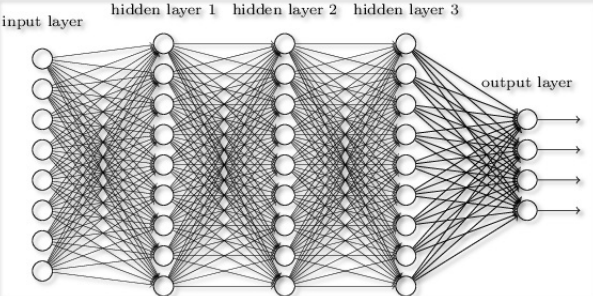
\includegraphics[scale=.7]{img/neuralNetwork.png}

\proposition{Function for Hidden Layers}
Below is a general function used to determine whether a neuron in a hidden layer is fired
$$z_j=h(a_j)\text{ where }a_j=\sum_{i=1}^Dw_{ji}x_i+w_{j0}$$
where $w_{ji}$ is the weight applied to the $i^{th}$ neuron by the $j^{th}$, $x_i$ is the value of the $i^{th}$ neuron, $w_{j0}$ is a bias \& $h(\cdot)$ is an activation function which acts to threshold $a_j$.\\

\proposition{Function for Ouptut Layer}
Whether a neuron on the \textit{Output Layer} is fired, to signal that this input should have this output, is determined by the below functions
$$y_k=f(a_k)=\sigma(a_k)\text{ where }a_k=\sum_{j=1}^Mw_{kj}z_j+w_{k0}$$
where $w_{kj}$ is the weight applied to the $j^{th}$ neuron by $k^{th}$, $w_{k0}$ is a bias and $z_j$ is the value of the $j^{th}$ neuron.\\

\proposition{Nesting Functions}
Since the functions for the \textit{Output Layer} depends on the vales on the hidden layers, and the hidden layers values depend on the previous layers to themselves it is clear to see how these functions become nested, composite functions.\\
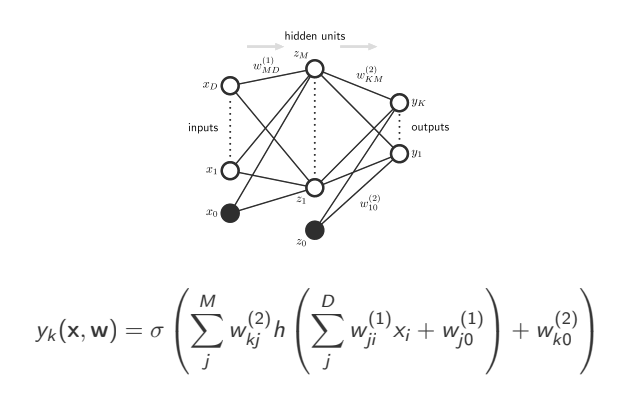
\includegraphics[scale=.8]{img/neuralNetworkFunction.png}

\definition{Kernel of a Function}
The \textit{Kernel} of a function is the set of values which map to themselves when the function is applied to them
$$\text{Ker}(f)=\{x\in X:f(x)=x\}\subseteq X\}$$

\definition{Image of a Function}
The \textit{Image} of a function is the set of all possible values which the function can output
$$\text{Im}(f)=\{y\in Y:\exists\ x\in X\text{ st }f(x)=y\}$$

\theorem{Rank-Nullity Theorem}
The \textit{Rank-Nullity Theorem} states that dimensionalities of the image and the kernel of a function will always sum to the dimensionality of the input space
$$\text{dim}(\text{Im}(f))+\text{dim}(\text{Ker}(f))=\text{dim}(X)$$

\proposition{Shrinking Image}
We can use the \textit{Rank-Nullity Theorem} and some intuition to realise that if we keep applying a function to itself its \textit{Image} will never grow and thus, the \textit{Kernel} can only grow.\\
The intuition here is that elements in the \textit{Kernel} can never leave it, by definition, by values may be mapped to a \textit{Kernel} value and thus leave the \textit{Image} and grow the \textit{Kernel}, where they are now stuck.\\

\remark{Usefulness of Shrinking Image}
By shrinking the \textit{Image} we are reduction what we are required to know, thus simplifying problems.\\

\theorem{Change of Variable}
Let $\x\in\mathcal{X}\subseteq\reals^n$ be a random vector with a probability density function given by $P_\X(\x)$ and let $\textbf{t}\in\mathcal{Y}\subseteq\reals^n$ be a random vector st $\phi(\textbf{y})=\x$ where $\pi:\mathcal{Y}\to\mathcal{X}$ is bijective and $|\nabla\phi(\textbf{y})|>0\ \forall\ \textbf{y}\in\mathcal{Y}$. Then the probabiltiy density funcyion $p_Y(\cdot)$ induced in $\mathcal{Y}$ is given by
$$p_Y(\textbf{y})=p_X(\phi(\textbf{y}))|\nabla\phi(\textbf{y})|$$
where $\nabla\phi(\cdot)$ denotes the Jacobian of $\phi(\cdot)$ and $|\cdot|$ denotes the determinant operator.\\

\proposition{Neural Network Learning}
\textit{Neural Networks} "Learn" by, first, \textit{Forward Propogation} where the hidden \& output layers apply their functions; then an error is calcualted for the set of weights, $W$, which were used during \textit{Forward Propogation}
$$E(W)=\sum_{i=1}^n\frac{1}{2}(g(\x_i,W)-y_i)^2+\text{reg}(W)$$
where $g(\cdot,\cdot)$ is the function which represents all the composite functions (here it outputs what the network belives the answer is), $y_i$ is the true result for $y_i$ and $\text{reg}(W)$ is %TODO
. The error is then back propogated to update the weights.\\

\definition{Backpropogation}
We update weights of neurons using by considering the gradient of the error (\ie how error changes between neurons).
$$W_t=W_{t-1}+\nu\frac{\partial}{\partial W}E(W)$$
where $\nu$ is the \textit{Learning Rate}.\\
We know the error on the output layer. The formula below allows us to propgate this eror back through the layers
$$\delta_\equiv\frac{\partial E_n}{\partial a_j}=\sum_k\frac{\partial E_n}{\partial a_k}\frac{\partial a_k}{\partial a_j}=\frac{\partial h(a_j)}{\partial a_j}\sum_jw_{kj}\delta_k$$
%TODO explain this

\propositionn{Process of Backpropagation}
\begin{enumerate}[label=\roman*)]
	\item Randomly initialise weights.
	\item Forward propogate.
	\item Compute Error.
	\item Compute gradients for one step back.
	\item Iteratively push gradients back.
	\item Update each layer.
	\item Repeat \textbf{ii)-vi)} until convergence
\end{enumerate}

\propositionn{Possible Acitvation Functions}
\begin{itemize}
	\item[-] Sigmoid, $f(x)=\dfrac{1}{1+e^{-x}}$
	\item[-] Tanh, $f(x)=\text{tanh}(x)=\dfrac{2}{1+e^{-2x}}-1$
	\item[-] ReLu, $f(x)=max(0,x)\approx\ln(1+e^x)$
\end{itemize}

\proposition{Neural Network Architectures}
There are many possible architectures for \textit{Neural Networks} and if we know \textit{a priori} then we can use that to reduce the search space.
\begin{itemize}
	\item[-] Convolution Neural Networks - Takes a weighted average within a spatial region (\ie blurring). Logic is that pixels depend on their neighbours.
	\item[-] Recurrent Neural Networks - Designed ot model sequential data
\end{itemize}

\remark{Neural Networks $\neq$ Models}
\textit{Neural Networks} are \textit{Decision Machines}, not \textit{Models}. This means they do not understand the data \& have no concept of uncertainty, thus new data cannot be generated from them. Further, random noise will always be assigned a label.\\

\propositionn{Combatting Limitations of Neural Networks being Decision Machines}
\begin{itemize}
	\item[-] Early stopping;
	\item[-] Layer-wise training;
	\item[-] Denoising;
	\item[-] Afverserial training;
	\item[-] Drop out
\end{itemize}

\section{Reinforcement Learning \& Decisions}

\definition{Reinforcement Learning}
\textit{Reinforcement Learning} tries to learn a solution without specifying the task explicitly, instead a system of providing awards for good actions is used.\\

\propositionn{Reinforcement Learning Process}
\begin{enumerate}[label=\roman*)]
	\item Agent takes an action in the environment.
	\item The environment changes as a result.
	\item The agent may be rewarded.
	\item Repeat \textbf{i)-iii)} until a time limit is reached
\end{enumerate}
\nb The strategy determined for the agent is called the \textit{policy}.\\

\remark{Optimal Behaviour wrt Time}
Different strategies are required to find an \textit{optimal behaviour} depending upon the time scale
\begin{itemize}
	\item[-] Finite time horizon, ${\displaystyle\expect\left(\sum_{t=0}^hr_t\right)}$
	\item[-] Average Reward (over all times), ${\displaystyle\lim_{h\to\infty}\expect\left(\frac{1}{h}\sum_{t=0}^hr_t\right)}$
	\item[-] Infinite Horizon (discounted reward) ${\displaystyle\expect\left(\sum_{t=0}^\infty\gamma^tr_t\right)}$ for $\gamma\in[0,1]$
\end{itemize}

\definition{Markov Decision Process}
Suppose we have a fully observable system we can determine the optimal policy using dynamic programming. \ie We know the \textit{Transition Matrix}, $T(s,a,s')$, and \textit{Reward Matrix}, $R(s,a,s')$, explicitly.
$$T(s,a,s')=\prob(s_{t+1}=s'|s_t=s,a_t=a)$$
$$R(s,a,s')=\expect(s_t=s,a_t=a,s_{t+1}=s')$$
where $s$ is the current state, $s'$ is another state \& $a$ is the action taken.\\

\remark{We might not be able to observe a state}

\proposition{Model Free}
Learning a mdel can be hard due to uncertainty propagation. Directly learning a function from state-action sets to reward can be easier
$$Q:\mathcal{S}\times\mathcal{A}\to\reals$$
\nb This does not build a model, rather a decision system.\\

\remark{Tricky part of Reinforcement Learning}
How to get the data.\\

\remark{Exploration v Explotation}
When thinking of a strategy to come up with a policy we need to balance: exploring the environement \& exploiting what we know.

\section{Classification}

\definition{Classification Task}
Consider a data set $\mathcal{D}$ where each item belongs to a class in $\mathcal{C}$.\\
The \textit{Classification Task} is given a set of observations $\{\mathcal{D,C}\}$ can we correctly associate new data to the correct classes?\\

\remark{Generative Models}
Suppose we have an image of a dog. The fact the appearance of image is a dog does not make the object a dog, the fact that the object is a dog makes the image have the appearance of a dog. Further we can have images that have the appearance of a dog but are not of a dog, such as drawings.\\

\remark{Classification is an Iverse Problem}
Further to \textbf{Remark 11.1} we note that multiple classes of objects can produce the same image. Thus when performing \textit{Classification} on an image we might need to return multiple possible classes.\\

\proposition{Formulating Classification}
Let $\x$ be a set of observed values \& $c_1\in\mathcal{C}$ is one of the possible classes we can assign to $\x$. By \textit{Bayes' Rule} we have
$$\prob(c_1|\x)=\dfrac{\prob(\x|c_1)\prob(c_1)}{\prob(\x)}$$
When the cardinality of $\mathcal{C}$ is low we can calculate the \textit{Evidence} explicitly
$$\prob(\x)=\sum_{c\in\mathcal{C}}\prob(\x|c)\prob(c)$$
Meaning the \textit{Posterior} can be formulatede as
$$\prob(c_1|\x)=\frac{\prob(\x|c_1)\prob(c_1)}{\sum_{c\in\mathcal{C}}\prob(\x|c)\prob(c)}$$

\proposition{Binary Classification}
Suppose we are classifying to one of two classes, \ie $\mathcal{C}:=\{c_1,c_2\}$. Then we have
\[\begin{array}{rrcl}
&\prob(\x)&=&\prob(\x|c_1)\prob(c_1)+\prob(\x|c_2)\prob(c_2)\\
\implies&\prob(c_1|\x)&=&\dfrac{\prob(\x|c_1)\prob(c_1)}{\prob(\x|c_1)\prob(c_1)+\prob(\x|c_2)\prob(c_2)}\\
&&=&\dfrac{\left(\frac{1}{\prob(\x|c_1)\prob(c_1)}\right)}{\left(\frac{1}{\prob(\x|c_1)\prob(c_1)}\right)}\dfrac{\prob(\x|c_1)\prob(c_1)}{\prob(\x|c_1)\prob(c_1)+\prob(\x|c_2)\prob(c_2)}\\
&&=&\dfrac{1}{1+\frac{\prob(\x|c_2)\prob(c_2)}{\prob(\x|c_1)\prob(c_1)}}\\
&&=&\dfrac{1}{1+\text{exp}\left(\ln\left(\frac{\prob(\x|c_2)\prob(c_2)}{\prob(\x|c_1)\prob(c_1)}\right)\right)}\\
&&=&\dfrac{1}{1+\text{exp}\left(-\ln\left(\frac{\prob(\x|c_1)\prob(c_1)}{\prob(\x|c_2)\prob(c_2)}\right)\right)}\\
&&=&\dfrac{1}{1+\text{exp}\left(-\ln\left(\frac{\prob(\x,c_1)}{\prob(\x,c_2)}\right)\right)}
\end{array}\]
We note the \textit{Sigmoid Function} has the form
$$y(t)=\frac{1}{1+e^{-t}}$$
By setting $t=\ln\left(\frac{\prob(\x,c_1)}{\prob(\x,c_2)}\right)$ we can use the \textit{Sigmoid Function} for \textit{Binary Classification}.\\

\proposition{Binary Classification - Gaussian}
In \textbf{Proposition 11.2} we did not specify the model for the data.\\
Suppose $\prob(\x|c_i)\sim_{Normal}(x|\mu_i,\sigma^2_i)$ then
\[\begin{array}{rrl}
t&:=&\ln\left(\frac{\prob(\x|c_1)\prob(c_1)}{\prob(\x|c_2)\prob(c_2)}\right)\\
&=&{\displaystyle\ln\left(\frac{\frac{1}{\sqrt{2\pi\sigma^2_1}}e^{-\frac{(\x-\mu_1)^2}{2\sigma^2_1}}\prob(c_1)}{\frac{1}{\sqrt{2\pi\sigma^2_2}}e^{-\frac{(\x-\mu_2)^2}{2\sigma^2_2}}\prob(c_2)}\right)}\\
&=&-\frac{1}{2}\ln\left(\frac{2\pi\sigma^2_1}{2\pi\sigma^2_2}\right)+\ln\left(\frac{\prob(c_1)}{\prob(c_2)}\right)-\frac{(x-\mu_1)^2}{2\sigma^2_1}+\frac{(x-\mu_2)^2}{2\sigma^2_2}\\
&=&\ln\left(\frac{\sigma_2}{\sigma_1}\right)+\ln\left(\frac{\prob(c_1)}{\prob(c_2)}\right)-x^2\left(\frac{1}{2\sigma_1^2}-\frac{1}{2\sigma_2^2}\right)+x\left(\frac{\mu_1}{\sigma_1^2}-\frac{\mu_2}{\sigma^2_2}\right)-\left(\frac{\mu_1^2}{\sigma_1^2}-\frac{\mu_2^2}{\sigma^2_2}\right)
\end{array}\]
We can analyse this expression of $t$ to see how the relationship between the distributions of $c_1$ \& $c_2$ affect classification.
\begin{enumerate}
	\item If $\sigma_1=\sigma_2$ the posterior is linear in $\x$.
	\item If $\mu_1=\mu_2$ and $\sigma_1=\sigma_2$ then the posterior is independent of $\x$ since $\prob(c_1|\x)=\prob(c_1)$
\end{enumerate}

\subsection{Logisitic Regression}

\definition{Logistic Regression}
\textit{Logisitic Regression} is a process of deriving an $f(\cdot)$ st
$$\prob(c_1|\x)=\frac{1}{1+e^{-f(\x)}}=\sigma(\x)$$
is a good binary classifier.\\
We aim to define $f(\cdot)$ such that objects in $c_1$ produced large \textit{positive} values \& objects in $c_2$ produce large \textit{negative} values.\\

\remark{Linear Classification}
If we use a \textit{Linear Classifier} with \textit{Logistic Regression} we define $f(\x)=\textbf{w}^T\x$ and our problem is to find $\textbf{w}$ which maximises positive values when $\x$ is of class $c_1$, and negative values when $\x$ is of class $c_2$.
$$\hat{\textbf{w}}_\text{MLE}=\text{argmax}_\textbf{w}\prob(\mathcal{C|D})=\text{argmin}_\textbf{w}-\ln\prob(\mathcal{C|D})$$

\remark{Usefullness of Logistic Regression}
If our feature data has high dimensionality then the mean \& co-variance matrices for each class will be high. This means that \textit{Classifiers} will have lots of parameters which need to be found. \textit{Logisitic Regression} requires only 1 more than the dimensionality of the feature data (a bias).\\

\example{Remark 11.4}
Suppose $\x\in\reals^{100}$ then each Gaussian $(\mu_i,\Sigma_i)$ would have dimensionality $\mu_i\in\reals^{100}\ \&\ \Sigma_i\in\reals^{100\times100}$. For a binary classifier this would require ${2(100+100\times100)=20200}$ parameters. Whereas a \textit{Logistic Regression} model requires $101$.\\

\remark{Limitations of Logistic Regression}
If a \textit{Logistic Regression} model is given an outlier point it will define it with almost absolute certainty to the class it is closest to. Other \textit{Models} which use a \textit{Gaussian} distribution will classify it to the same class as the \textit{Logistic Regression} model but with lower certainty as the two tails will have a similar value at the outlier.

\subsection{Laplace Approximation}

\definition{Laplace Approxmation}
\textit{Laplace Approximation} is used to approximate the integral of functions which have most their mass concentrated in a small area (and thus have rapidly decreasing tails).\\
Let $x_0:=\text{argmax}_xg(x)$ for some continuous function $g$.\\
Define $h(x):=\ln g(x)$. Then
\[\begin{array}{rcl}
\displaystyle\int_a^bg(x)dx&=&{\displaystyle\int_a^b\text{exp}(h(x)dx}\\
&\approx&{\displaystyle\int_a^b\text{exp}\left(h(x_0)+h'(x_0)(x-x_0)+\frac{1}{2}h''(x_0)(x-x_0)^2\right)dx\text{ by Taylor Expansion}}\\
\end{array}\]
Since we define $h(x_0)$ to be a maximum, $h'(x_0)=0$. Thus
$$\int_a^b\text{exp}(h(x))dx\approx\int_a^b\text{exp}\left(h(x_0)+\frac{1}{2}h''(x_0)(x-x_0)^2\right)$$
TODO - Read book on this

\section{Approximative Inference}

\definition{Markov Random Field}
A \textit{Markov Random Field} is a graph of random variables where edges show dependency between random variables.\\
Images can be considered as \textit{Markov Random Fields} as adjacent pixels depend upon each other.\\
\nb Also known as a \textit{Markov Network}.\\

\remark{Markov Random Field Marginal Likelihood}
Let $\{x_1,x_2,\dots\}$ be the set of all binary images \& $y$ be a class that an image can be assigned to. Then
$$\prob(y)=\int\prob(y|x)\prob(x)dx=\sum_i\prob(y|x_i)\prob(x_i)$$
\ie Integrating over all binary images. The number of possible binary images is finite so we can sum over it, but it is a big number so obviously a fouls errend.\\

\remarkk{Techniques for sampling from distributions we do not know the form of}
\begin{enumerate}[label=\roman*)]
	\item Rejection Sampling.
	\item Importance Sampling.
	\item Markov Chain Monte Carlo.
\end{enumerate}

\remark{}
Let $p(\cdot)$ be a distribution we do not know how to sample from \& $\tilde{p}(\cdot)$ be one we do
$$p(\cdot)=\frac{1}{Z}\tilde{p}(z)$$

\definition{Rejection Sampling}
\textit{Rejection Sampling} is a tecnique used to sample from distributions which we do not know explicitly.\\
Suppose $Z\sim f_Z(\cdot)$ is a distribution we do not know the form of.
\begin{enumerate}
	\item Pick an approximate distribution, $h_Z(\cdot)$.
	\item Choose a $k\in\reals^{\geq0}$ such that $kh_Z(z)\geq f_Z(z)\ \forall\ z$.
	\item Pick a random location using the approximate distribution $z_0\sim h_Z(\cdot)$.
	\item Pick a random number from the uniform distribution $u_0\sim\text{Uniform}[0,kh_Z(z_0)]$.
	\item If $u_0>f_Z(z_0)$ then reject $z_0$ otherwise sample it.
\end{enumerate}
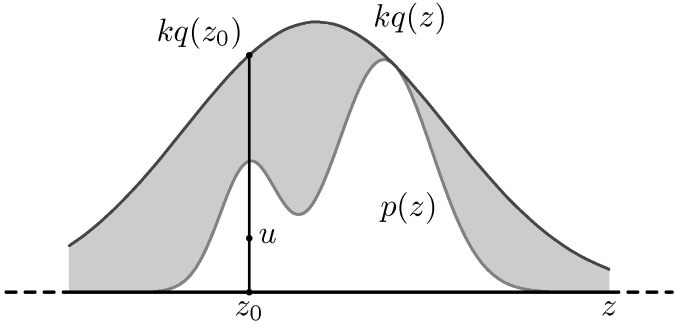
\includegraphics[scale=.4]{img/rejectionSampling.png}

\remarkk{Reject Sampling}
\begin{itemize}
	\item[-] We can use the distribution of the samples as a \textit{proposed distribution} for $f_Z$.
	\item[-] If the bound between $kh_Z$ and $f_Z$ is tight then the sampler is efficient. Often it is nt though as we have to set $k$ so high.
	\item[-] Does not scale well to multiple dimension.
	\item[-] Lots of samples get rejected.
\end{itemize}

\definition{Importance Sampling}
Suppose $Z\sim f_Z(\cdot)$ is a distribution we do not know the form of and $h_Z$ be a distribution we do know explicitly.\\
\textit{Importance Sampling} is a technique used estimate teh expected value of $Z$.
\[\begin{array}{rcl}
\expect_{\prob}(f_Z)&=&\int f_Z(z)\prob(z)dz\\
&=&\int f_Z(z)\prob(z)\frac{h_Z(z)}{h_Z(z)}dz\\
&=&\int f_Z(z)\frac{\prob(z)}{h_Z(z)}h_Z(z)dz\\
&=&\expect_{h_Z}\left(f_Z(z)\frac{\prob(z)}{h_Z(z)}\right)\\
&\approx&{\displaystyle\frac{1}{L}\sum_{i=1}^Lf_Z(z^{(i)})\frac{\prob(z^{(i)})}{h_Z(z^{(i)})}}\\
\end{array}\]
where $z^{(i)}\sim h_Z(\cdot)$.\\
TODO - pretty sure I am confused about $f_Z$ and $h_Z$.\\

\remarkk{Importance Sampling}
\begin{itemize}
	\item[-] Accepts all samples.
	\item[-] $\frac{\prob(z^{(i)})}{f_Z(z^{(i)})}$ corrects bias in sampling from the wrong distribution.
	\item[-] It is not always possible to evaluate $\prob(z)$.
\end{itemize}

\definition{Markov Chain Monte Carlo}
\textit{Markov Chain Monte Carlo} is a set of methods used for sampling from a probability distribution which is not known explicitly.\\
Let $z_t$ be the state at time $t$ and $h_Z(\cdot)$ be a proposed conditional distribution which we can sample from.
\begin{enumerate}
	\item Initialise a state $z_0$.
	\item Sample from the proposed conditional distribution $h_Z(z^*|z_0)$.
	\item Compute an acceptance probability
	$$A(z^*,z_0)=\min\left(1,\frac{\tilde{p}(z^*)}{\tilde{p}(z_0)}\right)$$
	\item Sample $u\sim\text{Uniform}(0,1)$.
	\begin{enumerate}
		\item If $A(z^*,z_0)$ >0 then $z_1=z^*$.
		\item Else $z_1=z_0$.
	\end{enumerate}
	\item Repeat 2-4 until time limit is reached.
\end{enumerate}

\example{Markov Chain Monte Carlo}
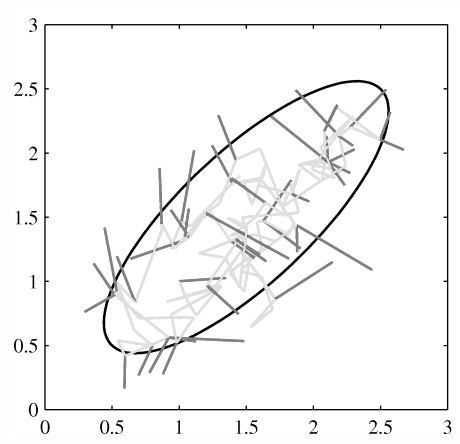
\includegraphics[scale=.4]{img/mcmc.png}

\remarkk{Markov Chain Monte Carlo}
\begin{itemize}
	\item[-] Has the \textit{Markov Property} - Remembers its state from the last sample \& uses it.
	\item[-] Good for exploration due to \textit{Markov Property}.
\end{itemize}

\definition{Gibbs Sampling}
\textit{Gibbs Sampling} exploits the fact that 1-dimension samples are often easy to get, in order to create a very simple markov chain.\\
\begin{enumerate}
	\item Intialise a state $\x_0$.
	\item Pick a single variable from that state, $x_i\in\x$.
	\item Formulate a posterior, $\prob(x_i|\x_{\neg i})$. $\x_{\neq i}$ is the state $x$ without variable $x_i$.
	\item Sample from the posterior
	$x_{(1,i)}\sim\prob(x_i|\x_{\neq i})$.
	\item Repeat 2-4 for all variables.
\end{enumerate}
\nb The general idea is to sample each variable in turn.

\newpage
\setcounter{section}{-1}
\section{Appendix}

\subsection{Definitions}

\definition{Memory-Based Methods}
\textit{Memory-Based Methods} for classification store the entire training set in order to make predictions for future data points. \eg Nearest-Neighbours.\\
\nb These generally require a distance measure to be defined.\\

\definition{Multinomial Distribution}
\textit{Multinomial Distribution} is a generalisation of the \textit{Binomial Distribution}.\\
It considers $n$ independent trials where each results in one of $k$ categories with the probability of each category being fixed.\\
$$\prob(\x;\textbf{p})=\begin{cases}\dfrac{n!}{x_1!\cdot\dots\cdot x_k!}p_1^{x_1}\cdot\dots\cdot p_k^{x_k},&\text{if }\sum_{i=1}^kx_i=n\\0&\text{otherwise}\end{cases}\text{ for }\x\in\reals^k$$
\nb Consider rolling a $k$ sided dice $n$ times

\subsection{Proofs}
\proof{Deriving Gaussian Marginal Distribution}
\textit{NOTE - This is dense as fuck \& uses quite a bit of bullshit}.\\
\\Let $\X\sim\mathcal{N}\left(\begin{pmatrix}
\mub_1\\\mub_2
\end{pmatrix},\begin{pmatrix}
\Lambda_{11}&\Lambda_{12}\\
\Lambda_{21}&\Lambda_{22}
\end{pmatrix}^{-1}\right)$.\\
$\mub_1,\mub_2$ can be considered as two parts of the mean vector $\mub$.\\
Let $\x$ be a realisation of $\X$ where $\x:=(\x_1,\x_2)$ with $\x_1\ \&\ \x_2$ representing the same partition as $\mub_1\ \&\ \mub_2$ respecitvely.\\
Define $D:=\mathrm{dim}(\x),\ D_1:=\mathrm{dim}(\x_1)\ \&\ D_2:=\mathrm{dim}(\x_2)$.\\
\\Here we want to get from $\prob(\x_1,\x_2)$ to $\prob(\x_1)$.\\
Consider the exponent of the joint distribution
$$E=-\frac{1}{2}(\x_1-\mub_1)^T\Lambda_11(\x_1-\mub_1)-\frac{1}{2}(\x_1-\mub_1)^T\Lambda_{12}(\x_2-\mub_2)-\frac{1}{2}(\x_2-\mub_2)^T\Lambda_{21}(\x_1-\mub_1)-\frac{1}{2}(\x_2-\mub_2)^T\Lambda_{22}(\x_2-\mub_2)$$
To produce the marginal for $x_1$ we want to isolate the terms involving $x_2$ so they are easy to remove.
\[\begin{array}{rcl}
E&=&-\frac{1}{2}\bigg[\left(\x_2^T\Lambda_{22}\x_2-2\x_2^T\Lambda_22(\mub_2-\Lambda_{22}^{-1}\Lambda_{21}(\x_1-\mub_1))\right)\\
&-&2\x_1^T\Lambda_{12}\mub_2+2\mub_1^T\Lambda_{12}\mub_2+\mub_2^T\Lambda_{22}\mub_2+\x_1^T\Lambda_{11}\x_1\\
&-&2\x_1^T\Lambda_11\mub_1+\mub_1^T\Lambda_{11}\mub_1\bigg]\\
&=&\underbrace{-\frac{1}{2}\left(\x_2-(\mub_2-\Lambda_{22}^{-1}\Lambda_{21}(\x_1-\mub_1))\right)^T\Lambda_{22}\left(\x_2-(\mub_2-\Lambda_{22}^{-1}\Lambda_{21}(\x_1-\mub_1))\right)}_{E_1}\\
&+&\underbrace{\frac{1}{2}\left(\x_1^T\Lambda_{12}\Lambda_{22}^{-1}\Lambda_{21}\x_1-2\x_1^T\Lambda_{12}\Lambda_{22}^{-1}\Lambda_{21}\mub_1+\mub_1^T\Lambda_{12}\Lambda_{22}^{-1}\Lambda_{21}\mub_1\right)}_{A}\\
&-&\underbrace{\frac{1}{2}\left(\x_1^T\Lambda_11\x_1-2\x_1^T\Lambda_{11}\mub_1+\mub_{1}\Lambda_{11}\mub_1\right)}_{B}
\end{array}\]
Note that $A$ \& $B$ do not contain any $x_2$ terms.\\
Since the co-variance matrix is symmetric we have $\Lambda_{12}=\Lambda_{21}^T$ we have
$$\x_1^T\Lambda_{12}\mub_2=\x_1^T\Lambda_{21}^T\mub_2=(\Lambda_{21}\x_1)^T\mub_2=\mub_2^T\Lambda_{21}\x_1$$
We shall not rewrite $A$ \& $B$ as quadratic expressions
\[\begin{array}{rrcl}
&A&=&\dfrac{1}{2}\left(\x_1^T\Lambda_{12}\Lambda_{22}^{-1}\Lambda_{21}\x_1-2\x_1^T\Lambda_{12}\Lambda_{22}^{-1}\Lambda_{21}\mub_1+\mub_1^T\Lambda_{12}\Lambda_{22}^{-1}\Lambda_{21}\mub_1\right)\\
&&=&\dfrac{1}{2}(\x_1-\mub_1)^T(\Lambda_{12}\Lambda_{22}^{-1}\Lambda_{21})(\x_1-\mub_1)\\
&B&=&\dfrac{1}{2}\left(\x_1^T\Lambda_{11}\x_1-2\x_1^T\Lambda_{11}\mub_1+\mub_{1}\Lambda_{11}\mub_1\right)\\
&&=&\dfrac{1}{2}(\x_1-\mub_1)^T\Lambda_{11}(\x_1-\mub_1)\\
\implies&A-B&=&\frac{1}{2}(\x_1-\mub_1)^T(\Lambda_{12}\Lambda_{22}^{-1}\Lambda_{21}-\Lambda_{11})(\x_1-\mub_1)\\
&\mathrm{Let\ }E_2&:=&A-B
\end{array}\]
Now the exponent has been orgainised we can consider the whole gaussian expression.
\[\begin{array}{rcll}
\prob(\x_1,\x_2)&=&\dfrac{e^{E_1}e^{E_2}}{(2\pi)^{\frac{D}{2}}|\Sigma|^{\frac{1}{2}}}\\
\prob(\x_1)&=&{\displaystyle\int\prob(\x_1,\x_2)d\x_2}\\
&=&{\displaystyle\int\dfrac{e^{E_1}e^{E_2}}{(2\pi)^{\frac{D}{2}}|\Sigma|^{\frac{1}{2}}}d\x_2}\\
&=&{\dfrac{e^{E_2}}{(2\pi)^{\frac{D}{2}}|\Sigma|^{\frac{1}{2}}}\displaystyle\int e^{E_1}d\x_2}&\text{Since $E_2$ is independent of $\x_2$}
\end{array}\]
Now we consider $\int e^{E_1}d\x_2$.\\
Since we know a gaussian must intergrate to 1 over the whole domain we deduce that
\[\begin{array}{rrcl}
&{\displaystyle\int\dfrac{1}{(2\pi)^{\frac{D_2}{2}}|\Lambda_{22}^{-1}|^{\frac{1}{2}}}e^{E_1}d_{\x_2}}&=&1\\\
\implies&\int e^{E_1}d\x_2&=&(2\pi)^{\frac{D_2}{2}}|\Lambda_{22}^{-1}|^{\frac{1}{2}}
\end{array}\]
\nb $\Lambda_{22}^{-1}$ is the variance of $\x_2$.\\
Using the result of this intergal we have
\[\begin{array}{rcl}
\prob(\x_1)&=&(2\pi)^{\frac{D_2}{2}}|\Lambda_{22}^{-1}|^{\frac{1}{2}}\dfrac{1}{(2\pi)^{\frac{D}{2}}|\Sigma|^{\frac{1}{2}}}e^{E_2}\\
&=&\dfrac{e^{E_2}}{(2\pi)^{\frac{D-D_2}{2}}|\Lambda_{22}^{-1}|^{-\frac{1}{2}}|\Sigma|^{\frac{1}{2}}}
\end{array}\]
The Schur complement of $\Lambda_{22}$ is $\Lambda^{-1}_{22}=\Sigma_{22}-\Sigma_{21}\Sigma_{11}^{-1}\Sigma_{12}$.\\
Thus \[\begin{array}{rcl}
|\Lambda_{22}^{-1}|^{-\frac{1}{2}}|\Sigma|^{\frac{1}{2}}&=&|\Sigma_{22}-\Sigma_{21}\Sigma_{11}^{-1}\Sigma_{12}|^{-\frac{1}{2}}|\Sigma_{11}|^{\frac{1}{2}}|\Sigma_{22}-\Sigma_{21}\Sigma_{11}^{-1}\Sigma_{12}|^{\frac{1}{2}}\\
&=&|\Sigma_{11}|^{\frac{1}{2}}
\end{array}\]
Now we have a full expression
\[\begin{array}{rcl}
\prob(\x_1)&=&\dfrac{e^{E_2}}{(2\pi)^{\frac{D-D_2}{2}}|\Lambda_{22}^{-1}|^{-\frac{1}{2}}|\Sigma|^{\frac{1}{2}}}\\
&=&\dfrac{1}{(2\pi)^{\frac{D_1}{2}}|\Sigma_{11}|^{\frac{1}{2}}}e^{-\frac{1}{2}(\x_1-\mub_1)^T\Sigma_{11}^{-1}(\x_1-\mub_1)}
\end{array}\]
\proved

\proof{Deriving Gaussian Conditional Distribution}
\\Let $\X\sim\mathcal{N}\left(\begin{pmatrix}
\mub_1\\\mub_2
\end{pmatrix},\begin{pmatrix}
\Sigma_{11}&\Sigma_{12}\\
\Sigma_{21}&\Sigma_{22}
\end{pmatrix}\right)$.\\
$\mub_1,\mub_2$ can be considered as two parts of the mean vector $\mub$.\\
Let $\x$ be a realisation of $\X$ where $\x:=(\x_1,\x_2)$ with $\x_1\ \&\ \x_2$ representing the same partition as $\mub_1\ \&\ \mub_2$ respecitvely.\\
Define $D:=\mathrm{dim}(\x)$.\\
\\We want to find the distribution of $\prob(\x_1|\x_2)$.\\
From the product rule we know that $\prob(\x_1,\x_2)=\prob(\x_1|\x_2)\prob(\x_2)$ and we already know the joint \& marginal distributions for a gaussian.\\
We have that
$$
\prob(\x_1,\x_2)\propto e^{-\frac{1}{2}\begin{pmatrix}
\x_1-\mub_1\\\x_2-\mub_2
\end{pmatrix}^T\begin{pmatrix}
\Sigma_{11}&\Sigma_{12}\\
\Sigma_{21}&\Sigma_{22}
\end{pmatrix}^{-1}\begin{pmatrix}
\x_1-\mub_1\\\x_2-\mub_2
\end{pmatrix}}$$
We now want to factor the marginal distribution out of this expression.
$$
\prob(\x_2)\propto e^{-\frac{1}{2}(\x_2-\mub_2)^T\Sigma_{22}^{-1}(\x_2-\mub_2)}
$$
Lets look at the exponent of the joint distribution.\\
\nb About to use a lot of Schur Complements
\[\begin{array}{rl}
E&=-\dfrac{1}{2}\begin{pmatrix}
\x_1-\mub_1\\\x_2-\mub_2
\end{pmatrix}^T\begin{pmatrix}
\Sigma_{11}&\Sigma_{12}\\
\Sigma_{21}&\Sigma_{22}
\end{pmatrix}^{-1}\begin{pmatrix}
\x_1-\mub_1\\\x_2-\mub_2
\end{pmatrix}\\
&=-\dfrac{1}{2}\begin{pmatrix}
\x_1-\mub_1\\
\x_2-\mub_2
\end{pmatrix}^T
\begin{pmatrix}
I&0\\
\Sigma_{22}^{-1}\Sigma_{21}&I
\end{pmatrix}^T
\begin{pmatrix}
(\Sigma/\Sigma_{22})^{-1}&0\\
0&\Sigma_{22}^{-1}
\end{pmatrix}
\begin{pmatrix}
I&-\Sigma_{12}\Sigma_{22}^{-1}\\
0&I
\end{pmatrix}
\begin{pmatrix}
\x_1-\mub_1\\
\x_2-\mub_2
\end{pmatrix}\\
&=-\dfrac{1}{2}\begin{pmatrix}
\x_1-\mub_1\\
\x_2-\mub_2
\end{pmatrix}^T
\begin{pmatrix}
(\Sigma/\Sigma_{22})^{-1}&-(\Sigma/\Sigma_{22})^{-1}\Sigma_{12}\Sigma_{22}^{-1}\\
-\Sigma_{21}\Sigma_{22}^{-1}(\Sigma/\Sigma_{22})^{-1}&\Sigma_{22}^{-1}
\end{pmatrix}^{-1}
\begin{pmatrix}
\x_1-\mub_1\\
\x_2-\mub_2
\end{pmatrix}\\
&=-\dfrac{1}{2}\bigg[\x_1-(\mub_1+\Sigma_{21}\Sigma_{22}^{-1}(\x_2-\mub_2))\bigg]^T(\Sigma/\Sigma_{22})^{-1}\bigg[\x_1-(\mub_1+\Sigma_{21}\Sigma_{22}^{-1}(\x_2-\mub_2))\bigg]\\
&\underbrace{-\dfrac{1}{2}(\x_2-\mub_2)^T\Sigma_{22}^{-1}(\x_2-\mub_2)}_{E_2}
\end{array}\]
Note that $E_2$ is exactly the exponent for the marginal distribution of $\x_2$ and thus what we want to factory out in order to get to the conditional distribution.
$$\prob(\x_1|\x_2)\propto e^{-\dfrac{1}{2}\big[\x_1-\underbrace{(\mub_1+\Sigma_{21}\Sigma_{22}^{-1}(\x_2-\mub_2))}_{\text{mean}}\big]^T(\underbrace{\Sigma/\Sigma_{22}}_{\text{covariance}})^{-1}\big[\x_1-(\mub_1+\Sigma_{21}\Sigma_{22}^{-1}(\x_2-\mub_2))\big]}$$
\proved
\subsection{Remarks}

\remark{Worlds}
We can consider 3 different when answering an ml question.
\begin{enumerate}[label=\roman*)]
	\item Deterministic, $x=4$;
	\item Point Estimate, $\text{argmax}_xp(x)=4$;
	\item Stochastic, $p(x)\sim\text{Normal}(4,10^2)$.
\end{enumerate}

\end{document}
